% Chapter Template

\chapter{Conclusion} % Main chapter title

\label{Chapter7} % Change X to a consecutive number; for referencing this chapter elsewhere, use \ref{ChapterX}

\lhead{Chapter 7. \emph{Conclusion}} % Change X to a consecutive number; this is for the header on each page - perhaps a shortened title

%----------------------------------------------------------------------------------------
%	SECTION 1
%----------------------------------------------------------------------------------------

\section{Summary of Important Points}
The aim of this thesis was to demonstrate how \ac{MRL} can be used to solve the symbol grounding problem in an unsupervised manner.

Through the course of the experiments shown in \autoref{Chapter4},5 and 6, I have demonstrated that the joint representation of different data modalities solves the symbol grounding problem. This was shown to be the case as the correct image was generated for each utterance provided in \autoref{Chapter4}. Similarly in \autoref{Chapter5} and \autoref{Chapter6} I showed that images of objects could be generated from their decriptions and vice-versa even for unseen combinations of attributes.

The learned representation has been demonstrated to fit the criteria layed out by Bengio et al. in \cite{repRev}. Particularly, the representation has been demonstrated to have Manifolds which can be manipulated through vector arithmetic to make predictable and meaningful changes in the output. For example, subtracting the representation of the word \textsc{red} from the representation of an image of a \textit{Red Triangle} and adding the representation of the word \textsc{Green} resulted in the generation of an image of a \textit{Green Triangle} in \autoref{Chapter5}. 

In some datasets, such as MNIST and ArtS, it is possible to generate image prototypes for each class/word in the \ac{MAE}'s ``vocabulary''. For MNIST, this came in the form of prototypical versions of each digit and for ArtS, images of each colour, shape and size can be generated individually.

This is also possible for the ReShape dataset However, due to the larger variability of training examples, the prototypes are very blurry. By using a class exemplar for each object, the \ac{MAE} was able to learn to generate non-blurry prototypes for each of the visual attributes.

I also demonstrated that \ac{MRL} can be used to generate accurate object descriptions of both real and artificial images. As well as that using \ac{MRL} can lead to improvements in classification accuracy as seen in \autoref{Chapter4} over unimodal baselines. However, this improvement comes at the cost of having worse performance when only a single modality is available.

In \autoref{Chapter5} and \autoref{Chapter6} I showed that \ac{MRL} allows \acp{ANN} to generalise to unseen objects. The \ac{MAE} is able to correctly generate images of objects which do not appear in the training data by combining the representations of different words. This entire process relies on the \ac{MAE} having grounded the meaning of each word individually to its image-space equivalent. The best example of this was the generation of a \textsc{Big Red Donut}.


\section{Conclusion}
\ac{MRL} has been shown to be a powerful technique and presents an area worthy of futher study. Whilst the findings of the experiments in this thesis are exciting, further work is needed to apply \ac{MRL} in a real world setting.

Unsupervised approaches to symbol grounding are vital to the development of robots for opperation in the real world. \ac{MRL} could form the foundation of a robotic cognitive system which can continue to learn throught its lifetime. Furthermore, the ability of the trained \acp{MAE} to generalise to unseen objects will make teaching robots about new objects quicker as it is not necessary to train the \ac{MAE} with every possible combination of visual attributes. Only a subset of attribute combinations needs to be learnt, from which other attribute combinations can be inferred as demonstrated in \autoref{Chapter5} when generating images of \textsc{Red Donuts}.



\section{Future Work}
The experiments layed out in the previous chapters have shown that \ac{MRL} using \acp{MAE} allows for the unsupervised learning of a grounded representation of images and language. How then, can this be used to improve robotic technologies?

I see many potential applications for \ac{MRL} within the field of \ac{HRI}. \autoref{fig:fsm} shows an example of how the \ac{MAE} can be included in a robotic system.


\begin{figure}
\centering
\includegraphics[width=\textwidth]{Figs/futureWork/fsm.png}
\caption{An example of how the \ac{MAE} can be used as part of a robotic system.}
\label{fig:fsm}
\end{figure}

Consider the scenario of a human interacting with a robot to teach it a set of objects and their visual attributes as well as the words used to describe the objects and their visual attributes. In a laboratory setting it is feasable to have only a single object in view at any given time. This is not true for real world scenarios. However, with the introduction of a \ac{FSM} controlled via a \ac{NLU} module, it is simple to use a \ac{MAE} trained with \ac{MRL} to discern which object is being referred to by the human. This is demonstrated in \autoref{fig:disamb}

\begin{figure}
\centering
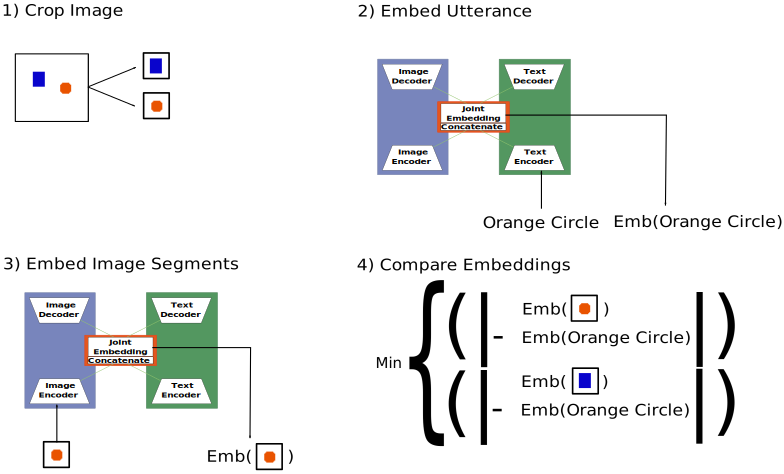
\includegraphics[width=\textwidth]{Figs/shapes/findingRefferant.png}
\caption{An example of using an MAE trained with MRL to disambiguate which object is being referred to in a scene.}
\label{fig:disamb}
\end{figure}

First, the image is split into patches, this can be done naively by sliding a window over the image and processing each patch. However this is not very computationally efficient and is likely to give ambiguous results, depending on the stride of the window, as multiple image patches may contain parts of the object of interest. Therefore it would be sensible to make use of an object detector such as Yolo v3 \cite{redmon2018yolov3} to predict object bounding boxes.

Comparing the embedding of each image patch to the embedding of the query, the image patch of interest should have the smallest \ac{MSE} between it and the query.

In order for the scenario depicted in \autoref{fig:disamb}, an \ac{NLU} module must be trained to extract the Intent of the human's utterance as well as any Entities which the human refers to. Fortunately, these types of \acp{NLU} are easily built using open source libraries like Rasa \cite{rasa}.



Developing the infrastructure for this type of scenario would allow for the exploration of questions such as:

\begin{itemize}
\item How many training examples does the \ac{MAE} require to operate accurately?
\item Is their an upper limit on the number of objects, visual attributes and words which the \ac{MAE} can learn?
\item How does regenerating a missing modality affect classification accuracy? Can the embedding of the regnerated missing modality be exploited to enhance  multimodal recognition techniques?
\end{itemize}

I believe \ac{MRL} can be used as a general tool for facilitating \ac{HRI} experiments, with the \ac{MAE} providing a piece of a cognitive architecture which translates low level sensory percepts (vision) to high level symbols (language).

\subsection{Accounting for time}
\textcolor{red}{Another way in which this system could be enhanced would to be to make use of recurrent encoders and decoders in the \ac{MAE} like those seen in \cite{gregor2015draw}. By allowing the \ac{MAE} to iteratively learn to represent data, it is posisble that a better representation of the data could be generated, which in turn would lead to better generation of images, text or sound. Further to this, such an extension might allow my approach to \ac{MRL} to be applied to time dependant problems like action or speech recognition.}


%-----------------------------------
%	SUBSECTION 1
%-----------------------------------


